\usepackage{xcolor}
\definecolor{PidInk}{HTML}{2C3E50}
\definecolor{PidIvory}{HTML}{F7F3E9}
\definecolor{PidLapis}{HTML}{1F3F60}
\definecolor{PidTeal}{HTML}{1F6968}
\definecolor{PidMineral}{HTML}{D2E0E2}
\definecolor{PidBronze}{HTML}{916400}
\definecolor{PidSaffron}{HTML}{B28218}
\definecolor{PidPomegranate}{HTML}{743E37}
\definecolor{PidSlate}{HTML}{647072}
\definecolor{PidPale}{HTML}{EDF5F3}
\definecolor{PidWarm}{HTML}{FBF5E8}

\pdfvariable minorversion=7
\usepackage{microtype}
\usepackage{fancyhdr}
\usepackage{titlesec}
\usepackage{enumitem}
\usepackage{booktabs}
\usepackage{longtable}
\usepackage{array}
\usepackage{ragged2e}
\usepackage{caption}
\usepackage{fvextra}
\usepackage{etoolbox}
\usepackage{needspace}
\usepackage{seqsplit}
\usepackage{xurl}
\usepackage{float}
\usepackage{tikz}
\usetikzlibrary{arrows.meta,calc,positioning}

\pagecolor{PidIvory}
\color{PidInk}
\raggedbottom
\clubpenalty=10000
\widowpenalty=10000
\displaywidowpenalty=10000
\setlength{\parindent}{0pt}
\setlength{\parskip}{0.46em plus .10em minus .07em}
\setlength{\emergencystretch}{10em}
\setlist{leftmargin=1.65em,itemsep=.20em,topsep=.30em,parsep=.05em}
\setlength{\LTpre}{.48em}
\setlength{\LTpost}{.70em}
\renewcommand{\arraystretch}{1.18}
\floatplacement{figure}{H}

\AtBeginEnvironment{longtable}{%
  \footnotesize\RaggedRight
  \setlength{\tabcolsep}{3.2pt}%
}
\captionsetup{font=small,labelfont={bf,color=PidTeal},textfont={color=PidInk},skip=7pt}

\DefineVerbatimEnvironment{Highlighting}{Verbatim}{
  breaklines,
  breakanywhere,
  commandchars=\\\{\},
  fontsize=\small,
  frame=single,
  framesep=4pt,
  rulecolor=\color{PidBronze}
}

\pagestyle{fancy}
\fancyhf{}
\fancyhead[L]{\footnotesize\color{PidInk}\bfseries PID2 represented-coordinate assurance}
\fancyhead[R]{\footnotesize\color{PidTeal}exact reduction · bounded guard · explicit limits}
\fancyfoot[L]{\footnotesize\color{PidSlate}pid-rs project analysis · 31 August 2026}
\fancyfoot[R]{\footnotesize\color{PidInk}\thepage}
\setlength{\headheight}{22pt}
\renewcommand{\headrulewidth}{0.25pt}
\renewcommand{\headrule}{\hbox to\headwidth{\color{PidBronze}\leaders\hrule height \headrulewidth\hfill}}
\fancypagestyle{plain}{%
  \fancyhf{}
  \fancyhead[L]{\footnotesize\color{PidInk}\bfseries PID2 represented-coordinate assurance}
  \fancyhead[R]{\footnotesize\color{PidTeal}mathematics, implementation, and nonclaims}
  \fancyfoot[L]{\footnotesize\color{PidSlate}pid-rs project analysis · 31 August 2026}
  \fancyfoot[R]{\footnotesize\color{PidInk}\thepage}
  \renewcommand{\headrulewidth}{0.25pt}
}

\titleformat{\section}
  {\Large\bfseries\color{PidInk}}
  {\thesection}{0.70em}{}
  [\vspace{.10em}{\color{PidBronze}\titlerule[.65pt]}\vspace{-.10em}{\color{PidSaffron}\titlerule[.20pt]}]
\titleformat{\subsection}{\large\bfseries\color{PidTeal}}{\thesubsection}{0.70em}{}
\titleformat{\subsubsection}{\normalsize\bfseries\color{PidTeal}}{\thesubsubsection}{0.70em}{}
\titlespacing*{\section}{0pt}{2.2ex plus .5ex}{1.0ex}
\titlespacing*{\subsection}{0pt}{1.8ex plus .4ex}{.8ex}
\titlespacing*{\subsubsection}{0pt}{1.5ex plus .3ex}{.7ex}

\renewenvironment{quote}
  {\par\vspace{.35em}\noindent{\color{PidBronze}\rule{\linewidth}{.55pt}}%
   \begin{list}{}{\leftmargin=3.5mm\rightmargin=3.5mm\topsep=.25em}%
   \item\relax\small\color{PidInk}}
  {\end{list}\noindent{\color{PidSaffron}\rule{\linewidth}{.20pt}}\par\vspace{.35em}}

\newcommand{\PidScopeFirewall}{%
  \begin{center}
  \begin{tikzpicture}[
    card/.style={draw=PidTeal,rounded corners=2mm,minimum height=30mm,text width=0.255\linewidth,
      align=left,inner sep=3.2mm,fill=PidPale,line width=.55pt},
    limit/.style={draw=PidPomegranate,rounded corners=2mm,minimum height=30mm,text width=0.255\linewidth,
      align=left,inner sep=3.2mm,fill=PidWarm,line width=.55pt},
    connector/.style={-{Stealth[length=2mm]},line width=.65pt,color=PidBronze}
  ]
    \node[card] (algebra) {\small\bfseries\color{PidTeal}EXACT-REAL ALGEBRA\\[1mm]
      \footnotesize Symbolic PID2 identities.\\Z3 plus substitution.};
    \node[card,right=8mm of algebra] (represented) {\small\bfseries\color{PidTeal}REPRESENTED\\COORDINATES\\[1mm]
      \footnotesize Selected binary64 contract.\\Integer/Fraction model plus compiled Rust.};
    \node[limit,right=8mm of represented] (science) {\small\bfseries\color{PidPomegranate}ESTIMATOR AND\\APPLICATION\\[1mm]
      \footnotesize Support, bias, calibration, and deployment need separate evidence.};
    \draw[connector] (algebra) -- node[above,font=\scriptsize,color=PidSlate] {complement} (represented);
    \draw[connector,dashed] (represented) -- node[above,font=\scriptsize,color=PidPomegranate] {no implication} (science);
  \end{tikzpicture}
  \end{center}
  \vspace{.2em}
}

\makeatletter
\renewcommand{\maketitle}{%
  \hypersetup{pageanchor=false}%
  \begin{titlepage}
    \thispagestyle{empty}
    \pagecolor{PidIvory}\color{PidInk}
    \begin{tikzpicture}[remember picture,overlay]
      \fill[PidLapis] (current page.north west) rectangle ([yshift=-116mm]current page.north east);
      \foreach \x in {0,1.7,...,22} {
        \foreach \y in {0,-1.7,...,-12} {
          \begin{scope}[shift={([xshift=\x cm,yshift=\y cm]current page.north west)},opacity=.16]
            \draw[PidMineral,line width=.35pt] (0:.66) -- (45:.94) -- (90:.66) -- (135:.94) -- (180:.66) -- (225:.94) -- (270:.66) -- (315:.94) -- cycle;
            \draw[PidMineral,line width=.25pt] (-.66,0)--(.66,0) (0,-.66)--(0,.66) (-.47,-.47)--(.47,.47) (-.47,.47)--(.47,-.47);
          \end{scope}
        }
      }
      \fill[PidTeal] ([yshift=-116mm]current page.north west) rectangle ([yshift=-111mm]current page.north east);
      \fill[PidBronze] ([xshift=18mm,yshift=24mm]current page.south west) rectangle ([xshift=-18mm,yshift=24.7mm]current page.south east);
    \end{tikzpicture}
    \vspace*{15mm}
    {\small\bfseries\color{PidMineral}\MakeUppercase{pid-rs numerical assurance volume}\par}
    \vspace{18mm}
    \begin{minipage}{0.92\textwidth}
      \RaggedRight
      {\fontsize{31}{37}\selectfont\bfseries\color{PidIvory}%
        \mbox{PID2 represented-coordinate}\par
        \mbox{assurance}\par}
    \end{minipage}\par
    \vspace{12mm}
    {\Large\bfseries\color{PidMineral}Exact binary64 reduction, guard boundaries, and evidence limits\par}
    \vspace{44mm}
    {\small\bfseries\color{PidTeal}\MakeUppercase{represented inputs · exact dyadics · explicit nonclaims}\par}
    \vspace{8mm}
    \begin{minipage}{0.88\textwidth}
      \large
      A self-contained account of the two-source reconstruction algebra, the selected binary64
      arithmetic contract, exact witnesses and counterexamples, conditioning outcomes, checker
      architecture, resource bounds, negative results, and remaining proof obligations.
    \end{minipage}\par
    \vfill
    \begin{minipage}{0.90\textwidth}
      \small\color{PidSlate}
      The integer-and-Fraction route is separately implemented: it differs from production in
      language, representation, and algorithm, but it is not independent estimation, external
      replication, or independent review.
    \end{minipage}\par
    \vspace{11mm}
    {\large\color{PidInk}\@date\par}
    \vspace{3mm}
    {\small\color{PidSlate}Canonical source: \texttt{PID2\_REPRESENTED\_COORDINATE\_ASSURANCE.md}\par}
    \vspace{17mm}
  \end{titlepage}
  \hypersetup{pageanchor=true}%
  \setcounter{page}{1}%
  \pagecolor{PidIvory}\color{PidInk}
}
\makeatother
